\documentclass[3p,twocolumn]{elsarticle}

\usepackage[utf8]{inputenc}
%\usepackage[polish]{babel}
%\usepackage{polski}
\usepackage{lineno,hyperref}
\modulolinenumbers[5]

\journal{Radosław Łazarz Journal}

%%%%%%%%%%%%%%%%%%%%%%%
%% Elsevier bibliography styles
%%%%%%%%%%%%%%%%%%%%%%%
%% To change the style, put a % in front of the second line of the current style and
%% remove the % from the second line of the style you would like to use.
%%%%%%%%%%%%%%%%%%%%%%%



%% Numbered
%\bibliographystyle{model1-num-names}

%% Numbered without titles
%\bibliographystyle{model1a-num-names}

%% Harvard
%\bibliographystyle{model2-names.bst}\biboptions{authoryear}

%% Vancouver numbered
%\usepackage{numcompress}\bibliographystyle{model3-num-names}

%% Vancouver name/year
%\usepackage{numcompress}\bibliographystyle{model4-names}\biboptions{authoryear}

%% APA style
%\bibliographystyle{model5-names}\biboptions{authoryear}

%% AMA style
%\usepackage{numcompress}\bibliographystyle{model6-num-names}

%% `Elsevier LaTeX' style
\bibliographystyle{elsarticle-num}
%%%%%%%%%%%%%%%%%%%%%%%

\begin{document}

\begin{frontmatter}

\title{Implementation of a neural network in C++ programming language using Armadillo library}
%\tnotetext[mytitlenote]{Fully documented templates are available in the elsarticle package on %\href{http://www.ctan.org/tex-archive/macros/latex/contrib/elsarticle}{CTAN}.}

%% Group authors per affiliation:
\author{Michał Hamuda}
\ead{hamud94@gmail.com}


\author{Paweł Nowak}
\ead{mail@mail}

\author{Mateusz Windak}
\ead{mail@mail}

%% or include affiliations in footnotes:


\begin{abstract}
In this article, we present our own implementation of a simple neural network for a classification problem using open source library for matrix calculations - Armadillo. The goals of this article are the following: firstly, to gain understanding what the neural networks really are - many people think of them as some mystcal, omnipotent, brain-like black-boxes, when in fact we show that a neural network in a basic form is just a series of matrices and a series of operations defined on them. Secondly, we want to examine if Armadillo library, and C++ language in general, can be a useful tool for machine-learning related programming. Python and R had became de facto industry standard in that field, but they both have their limitations, so it is worthwhile to seek for alternatives. And, last but not least, our third goal when writing this article is to obtain 5 points needed by us to pass the famous MRO course, the last course standing between us and the engineer's degree.
\end{abstract}

\begin{keyword}
\texttt{Armadillo} \sep C++ \sep neural network \sep MRO
\end{keyword}

\end{frontmatter}

%\linenumbers

\section{The problem}

The problem that our network attempts to solve is the famous classification problem. In this problem, we have an n-dimensional space where each point belongs to one of the $k$ classes. We do not have full knowledge about class membership - in fact we have a training set $T$ containing finite number of points, and only for the points from T we know which class they belong to. What this problem wants us to do is to construct a program that would take as an input $x$ and $T$, where $T$ is the training set, and $x$ is any point from the space, and as an output determine to which class does the $x$ belong.

Such definition might sound very dry and mathematical, like the jargon that the scientists use to be perceived as more intelligent than everyone else, but let's show it on a real world example: election statistics. Suppose we have a two-dimesional space representing people. One dimension is the age, second dimension is the income level. Our classes will be political preferences - one class will be people supporting party A and the second class will be people supporting party B, because for some reason, we believe that age and income level is correlated with political preferences, so people of certain age and certain incomes will support party A, and people of different age and income will support party B. We believe that such correlation exists, but we don't know how does it exactly look like - in fact all we know is some set of people T, that we have actually reached out and asked such indiscrete questions like how old are you, how much do you earn and who do you vote for. What we want to do is to take the information from the set T and build a program that for any combination of age and income would tell us on which side of the barricade this combination is. We want to be able to create plot as in Figure \ref{fig:fig1}

\begin{figure}[h]
	
\label{fig:fig1}
  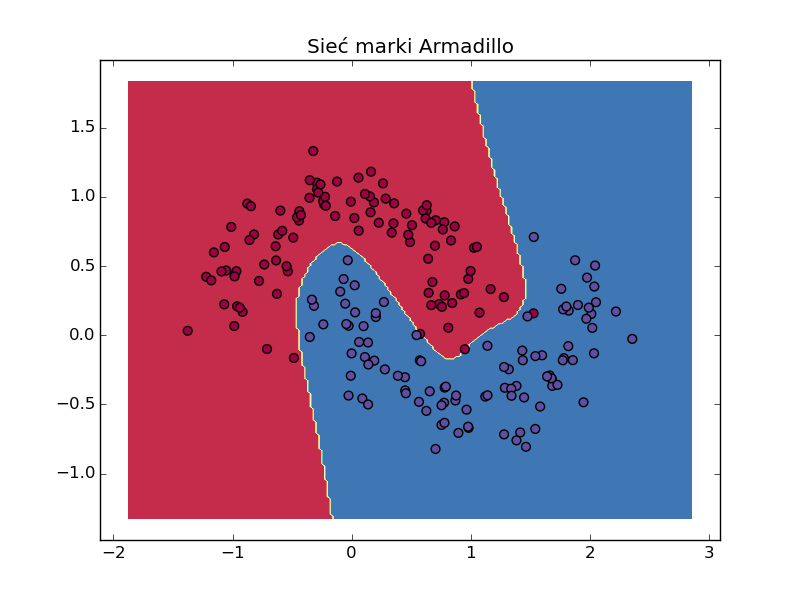
\includegraphics[width=\linewidth]{figure_1.png}
	\caption{Political preferences - colors represent parties, points form the set T}
	\label{fig1}
\end{figure}


\section{The solution}

How do we want to tackle that problem? We are going to use machine learning. First, we will come up with a function with some parameters and we will assume that this function can approximate the output we want to get, and using the training set we will try to find optimal values of the parameters - optimal in the sence that with them function gives the best approximation.

So, what will be our parametrized function? Let us summon a mathematical abstraction called neural network. Basic building block of a neural network is a perceptron - a function that takes a vector as an input and produces a single scalar as an output. Input of one perceptron can consist of outputs of other perceptrons - therefore perceptrons can be connected forming a directed graph called \emph{the net}. The net is usually aligned into layers - input layer, one or more hidden layers, and output layer, as shown in Figure \ref{fig2}. In such aligment, we can treat the whole \emph{layer} as a function that takes a matrix as an input and produces some other matrix as an output, and output of one layer becomes input of another. How does the perceptron - and therefore the layer compute output? Perceptron has a vector of weights $W$ a free term $b$, and an arbitrary \emph{activation function} $s$ needed to introduce nonlinearity. It takes input vector $x$, computes scalar product with $W$, adds the free term $b$, and passes that through the activation function. Generalizing, the \emph{layer} has a \emph{matrix} of weights $W$ and a \emph{vector} of free terms $b$ and the activation function. So, the formula for the output is the following:

\[ y = s(Wx + b) \]

In our case - the classification problem - the input of the first layer will be $n$-dimensional vector of the point coordinates, and the output of the last layer will be $k$-dimensional vector where the i-th element will be the probability that the point belongs to the i-th class. The acitivation function is chosen arbitrarily - we chose $tanh$ - and W and b matrices of each layer are the parameters whose values we want to find. We find them by first assigning random values to them and then iteratively trying to improve them. What follows is a philosophical question: what does it mean to improve something? What does it mean to improve parameters? Is improvement something that can be measured or is it a matter of subjective feeling, perceived differently by every person? It turns out that in case of parameters, it can be measured. To do that, we introduce \emph{loss function} that will take as an input a points with known classifications and our whole network and will produce a single number saying how well does our net perform on this set of points, i.e. what is the percentage of points for which our net incorrectly guesses class membership. Therefore, when we iteratively try to improve parameters, we want to find new parameters for which the loss function of the net will be lower than for the previous ones. For that we use method called \emph{gradient descent} -  we compute gradients of the loss function with respect to the parameters ( $\frac{\partial L}{\partial W_1}$, $\frac{\partial L}{\partial b_1}$ and so on) and we 'move' the parameters in direction of those gradients therefore iteratively approaching the local minimum of the loss function. That of course means that depending on how we (randomly) choose initial values of the parameters we can get stuck in the local minimum and never achieve the global minimum that can be just few steps away. But well, that's life, nobody said it will be all pink and roses.

\begin{figure}[h]
	
\label{fig:fig2}
  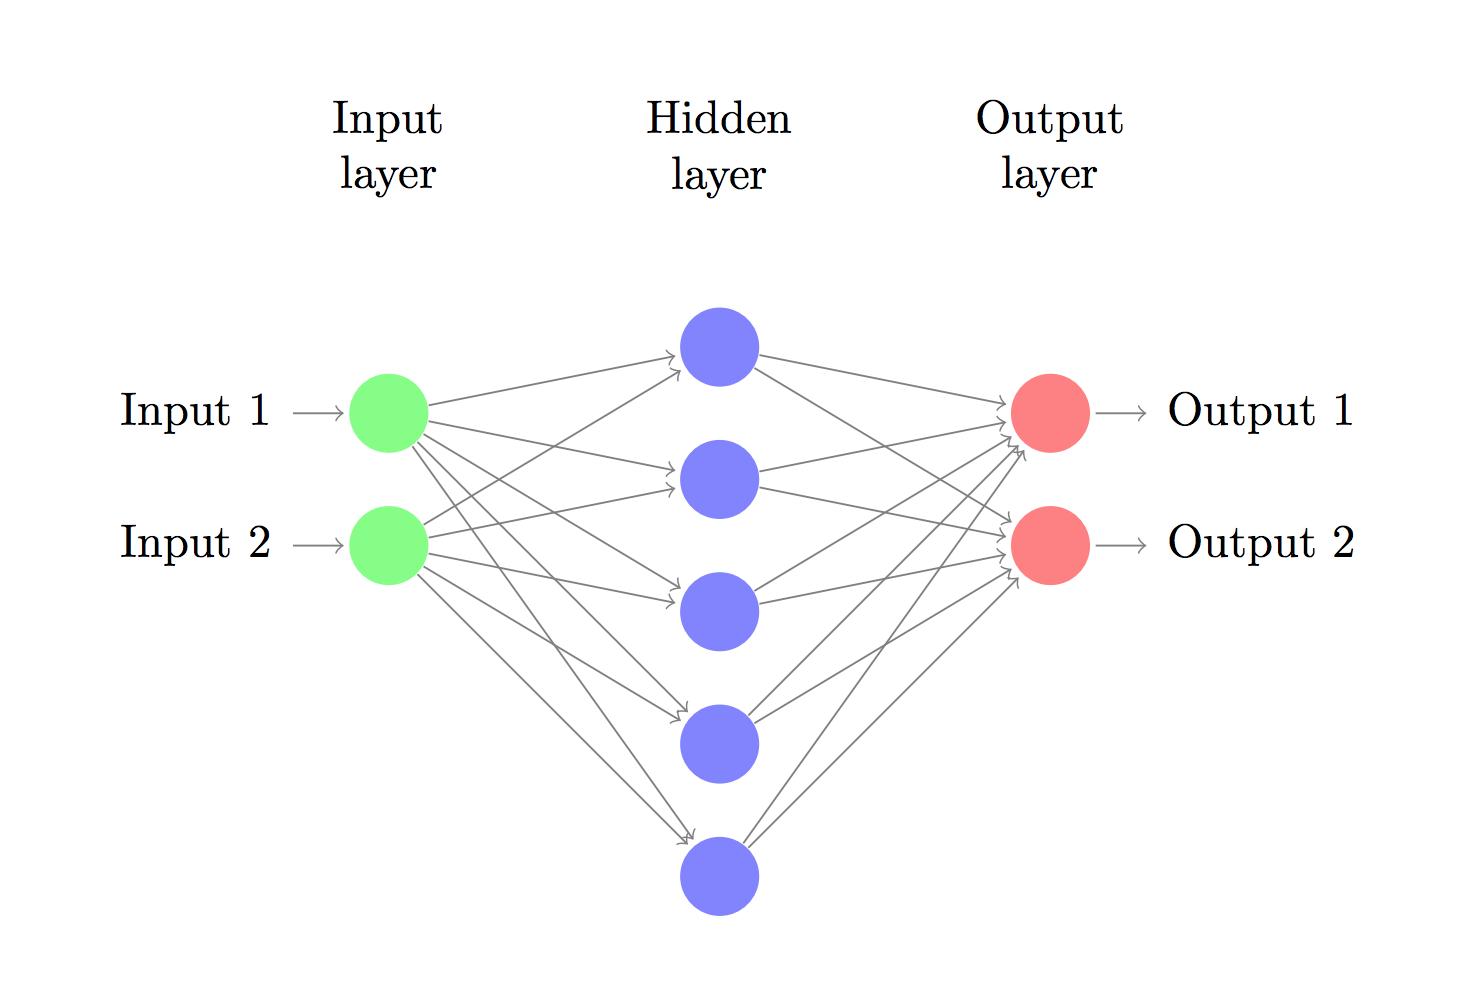
\includegraphics[width=\linewidth]{network-schema.png}
	\caption{Schema of the neural network}
	\label{fig2}
\end{figure}

\section{The implementation}

One of the advantages of the C++ language is its strong type system. It makes it much easier working with legacy code or with a library previously unknown to the programmer, because types alone can give a lot of information about what a given method or class is actually doing. We wanted to follow that path and we wanted our implementation to have types reflecting the mathematical model we described above. Armadillo provided us with classes for matrix and vector - \emph{mat} and \emph{rowvec}, what we have to do was to implement classes representing layer of the network and the whole network. (Actually we could also model perceptron as a separated class, but we decided not to do it as it would be too detalistic and would make things more complex and not more simple). Diagram of our classes with their interfaces can be seen on Figure \ref{fig:fig1} We designed the model in such way that it can support any size of input and output vector and any number of layers, however we used it only for input and output vectors of size two and three layers. It was proven that there is no point to further increase the number of layers, because any multi-layer network can be simulated on a three-layer one. (Except for a more advanced type of networks, called \emph{convolutional neural networks}, but that is a whole different story).

\begin{figure}[h]
	
\label{fig:fig3}
  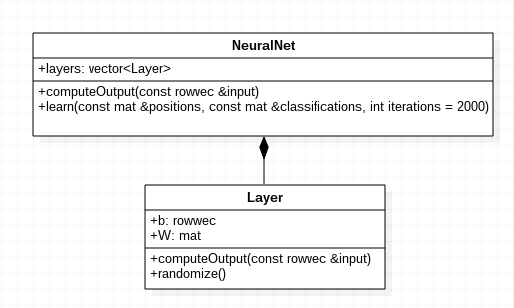
\includegraphics[width=\linewidth]{uml-diagram.png}
	\caption{UML diagram of our implementation (library classes not shown)}
	\label{fig3}
\end{figure}

\section{The results}

There is a danger that casts its shadow over all the machine learning and human learning as well. This danger is called \emph{overfitting}. It means that if a net, a method, a program, a human is trained only on a data from one training set it might become too adjusted to the training set so it will perform well on input from the training set, but perform poorly on any other input. To take this into account, a common practise in machine learning is to firstly generate a data set, and divide it randomly into two or more sets - first set will be training set, second will be test set. Other ones can be test or validation sets, according to the needs. The method is trained using the training set, and then the test set is used to measure how good the method actually is and if it can grasp the characteristics and regularities present it the whole data set, not only in the chunk of it that was passed as the input of the method. In our experiments, we wrote a Python script that generated for us data set of 1000 points divided into two classes (using function \texttt{sklearn.datasets.make\_moons} from the \texttt{scikit-learn} package), divided it randomly into 700-point training set and 300-point test set, and then finally saved them to csv files. Our C++ program with the neural net took those csv files as the input and produced its output also as a csv file. The form of the output that could be then plotted was a grid of evenly spread points together with their predicted classifications. This output was then read by another Python script that used \texttt{pyplot} package to generate png image with the plot. The results can be seen on Figures 4-10 - 'nodes' is the number of perceptrons in the hidden layer, 'quality' is the percentage of correct classifications in the test set, and epsilon and lambda are arbitrary parameters of the neural net. In gradient descent, epsilon determines how big should be the step in the direction pointed by the gradient, and lambda is the coefficient of the regularisation term introduced to prevent overfitting. We experimented with different values of epsilon and lambda, as well as with different amount of nodes. Experiments demonstrated that the optimal value of both epsilon and lambda is 0.01, other values can give catastrophic results. In the case of the number of nodes, choosing optimal value isn't so simple - it is always a tradeoff. Number of nodes determines how complex the decision boundary can be - when number of nodes is small, the boundary is almost linear (for two nodes it is exactly linear), when number of nodes is biger, the boundary can be more curved and irregular. So, when we choose number of nodes for our net 



\begin{figure}[h]
\label{fig:fig4}
  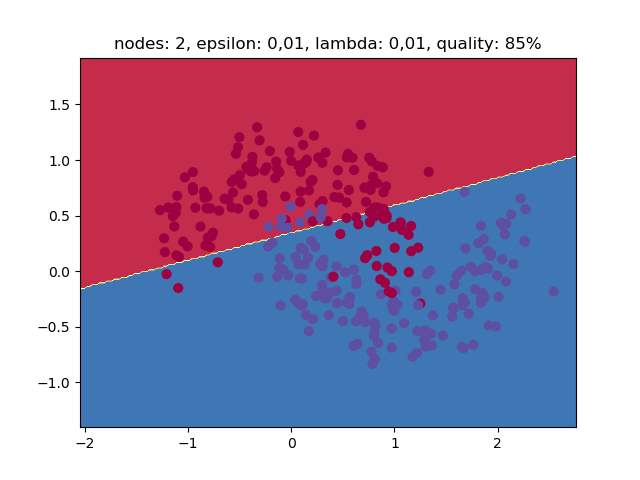
\includegraphics[width=\linewidth]{wykresy/1.png}
	\caption{Result of our net - for two-node hidden layer separation of classes is almost linear}
	\label{fig4}
\end{figure}

\begin{figure}[h]
\label{fig:fig4}
  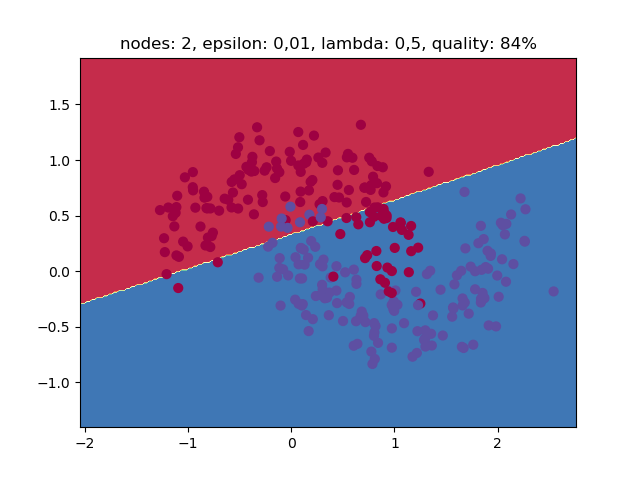
\includegraphics[width=\linewidth]{wykresy/2.png}
	\caption{Increasing value of lambda doesn't result in much change...}
	\label{fig4}
\end{figure}

\begin{figure}[h]
\label{fig:fig4}
  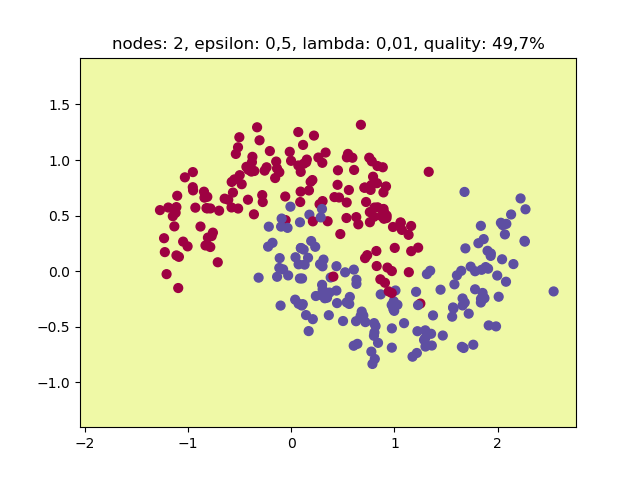
\includegraphics[width=\linewidth]{wykresy/5.png}
	\caption{But increasing epsilon does - the net becames useless assingning all points to the same class}
	\label{fig4}
\end{figure}

\begin{figure}[h]
\label{fig:fig4}
  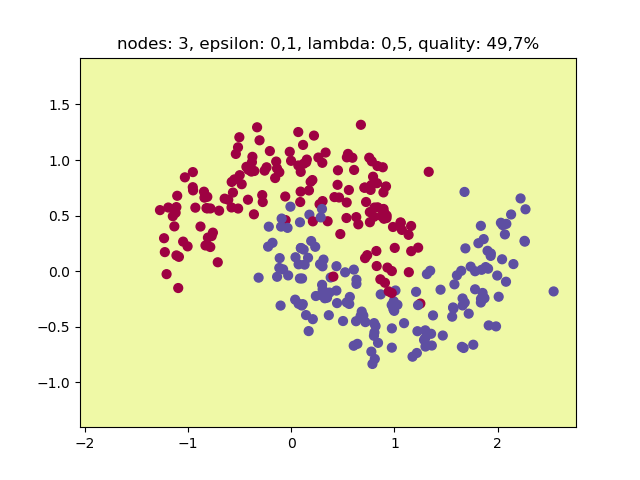
\includegraphics[width=\linewidth]{wykresy/10.png}
	\caption{It turns out that changing the lambda sometimes is effectless and sometimes it isn't.}
	\label{fig4}
\end{figure}

\begin{figure}[h]
\label{fig:fig5}
  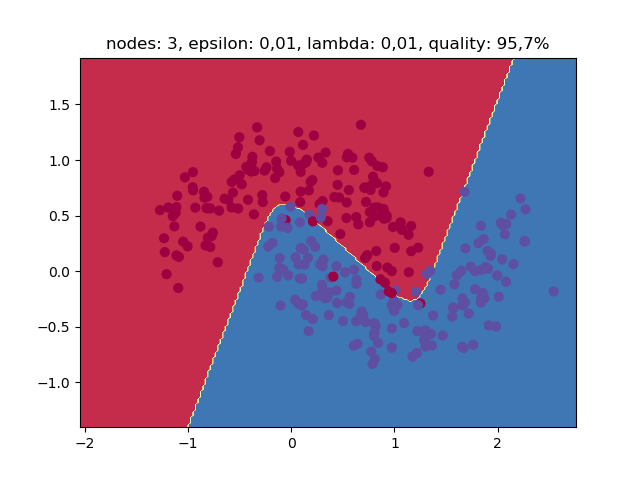
\includegraphics[width=\linewidth]{wykresy/7.png}
	\caption{ Increasing number of nodes from 2 to 3 gives much improvement}
	\label{fig5}
\end{figure}

\begin{figure}[h]
\label{fig:fig5}
  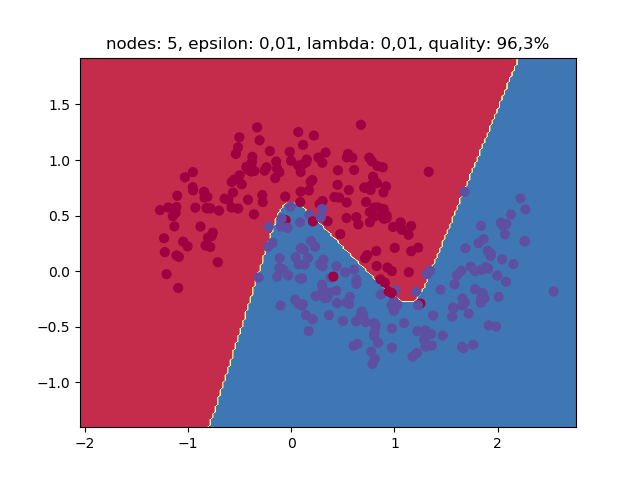
\includegraphics[width=\linewidth]{wykresy/13.png}
	\caption{ Five nodes - almost like three}
	\label{fig5}
\end{figure}

\begin{figure}[h]
\label{fig:fig5}
  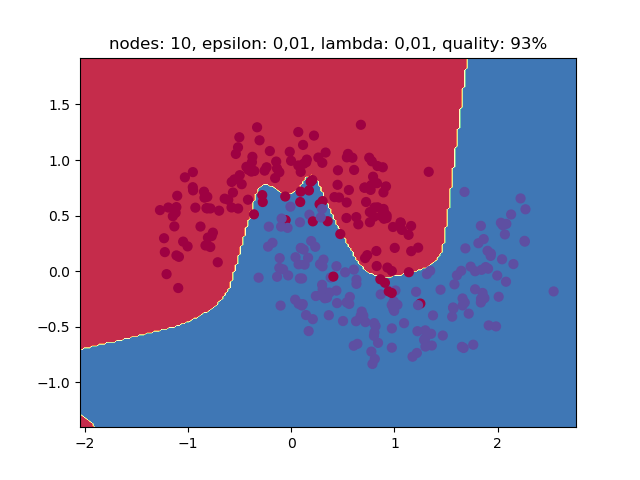
\includegraphics[width=\linewidth]{wykresy/19.png}
	\caption{ Ten nodes - irregularities begin, quality of prediction decreases}
	\label{fig5}
\end{figure}

\begin{figure}[h]
\label{fig:fig5}
  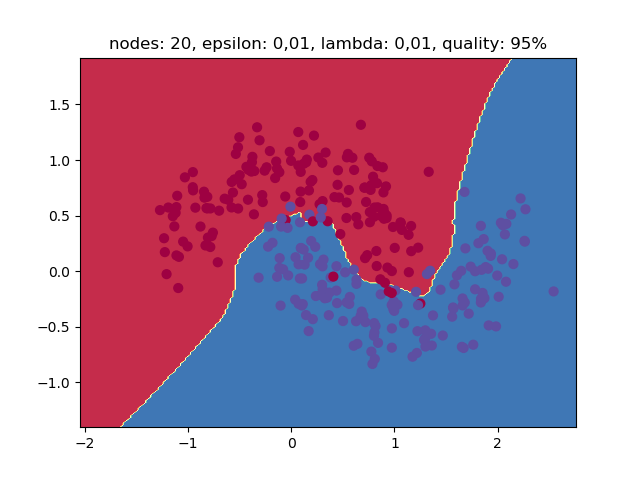
\includegraphics[width=\linewidth]{wykresy/20.png}
	\caption{ Twenty nodes - quality improves a little bit, but does not reach the previous level}
	\label{fig5}
\end{figure}

\begin{figure}[h]
\label{fig:fig5}
  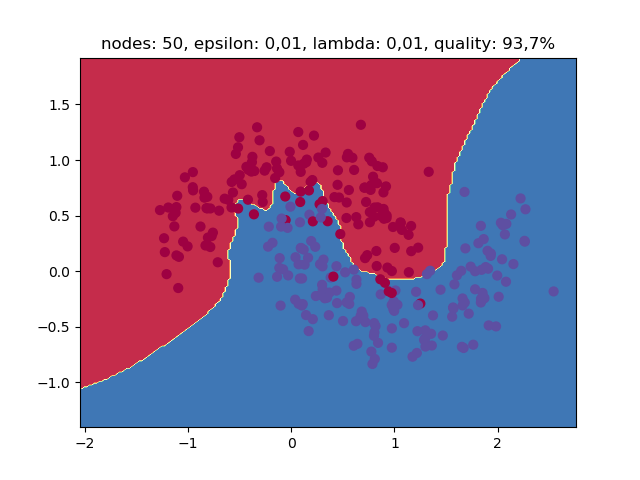
\includegraphics[width=\linewidth]{wykresy/21.png}
	\caption{ Fifty nodes - more irregularities, quality decreases again}
	\label{fig5}
\end{figure}

\section{The summary}


%\bibliography{mybibfile}

 \begin{thebibliography}{00}

% \bibitem must have the following form:
%   \bibitem{key}...
%

 \bibitem{armadillo} Armadillo homepage http://arma.sourceforge.net
 
 \bibitem{stack} Stack overflow

 \end{thebibliography}

\end{document}
